\section{Reactive Extensions}
There have been many attempts to fit the philosophy of reactive programming into frameworks, APIs and even languages \cite{ReactiveX, meijer2015-Dart, Reactive-Streams, Akka, Elm, RxMobile}. In this section, we will discuss some of the features of one of these libraries, namely Reactive Extensions (a.k.a. Rx). This project started at Microsoft with an implementation in C\# \cite{meijer2010-Observable} (Rx.Net), was later ported to Java, Scala, Groovy, Kotlin, JavaScript, Swift and many other languages by the open source community \cite{ReactiveX}. It is currently the standard library for programming in a reactive way.

Unfortunately, these various translations have each been evolving in their own way, deviating from both the original implementation as well as each other. There are obvious minor changes such as operator names changing to conform particular language standards, but also behavior in various corner cases changed. Most remarkable however is that some implementations are not even purely `reactive' anymore \cite{meijer2014-Derivation}. Given these deviations from the original paradigm and the state of complexity of these implementations, we decided to use a reference implementation of the original Rx that has recently been written in Scala by Erik Meijer et al. called RxMobile \cite{RxMobile}, with the purpose of creating a light-weight implementation for mobile app development. The following discussion and derivation of the API will however apply to both Reactive Extensions and RxMobile and in this section we will therefore refer to both of them as `Rx'.

\subsection{Core components}
\label{subsec:core-comps}
Rx is a library for composing asynchronous and event based (reactive) programs by using observable sequences \cite{Rx-Codeplex}. The core of Rx consists of two interfaces: \obs and \obv. The latter can subscribe and react to the events that are emitted by the former. An \obs can emit zero or more events (called \textit{onNext}) and has the possibility to terminate with an \textit{onCompleted} or \textit{onError} event. After either one of these terminal events is emitted, no more events can follow. Therefore the emission protocol can be summarized by the following regular expression: \code{onNext* (onError | onCompleted)?} \cite{MS2010-RxDesign}. When an \obv subscribes to an \obs, it will return a \subs. With this object reference, one can later unsubscribe from the \obs and clean up potential resources.

\Cref{lst:obs-obv} shows these basic concepts of the \obs, \obv and \subs translated in Scala. Notice that here \subs is a superclass of \obv. Therefore there is no need for the \obs to return a \subs when an \obv subscribes to it. It will however return a \subs when another variant of \code{subscribe} is used, where for example a lambda expression is expected instead.

Creating an \obs is done by the \code{Observable.create(Observer $\Rightarrow$ Unit): Observable} method, that takes a lambda expression of type \code{Observer $\Rightarrow$ Unit} and returns an \obs. The input lambda is then used in the implementation of \code{subscribe}, when a \emph{real} \obv is provided. The \obv can be created by supplying it three lambda expressions, one for each kind of event.

\begin{minipage}{\linewidth}
\begin{lstlisting}[style=ScalaStyle, caption={Observable, Observer and Subscription}, label={lst:obs-obv}]
trait Observable[T] {
    def subscribe(observer: Observer[T]): Unit
    def subscribe(onNext: T $\Rightarrow$ Unit): Subscription
    // other variants of subscribe
}
object Observable {
  def create[T](create: Observer[T] $\Rightarrow$ Unit) $=$ new Observable[T] {
    override def subscribe(observer: Observer[T]) $=$ create(observer)
  }
  // other ways to create an Observable
}

trait Observer[T] extends Subscription {
    def onNext(t: T): Unit
    def onError(e: Throwable): Unit
    def onCompleted(): Unit
}

trait Subscription {
    def isUnsubscribed(): Boolean
    def unsubscribe(): Unit
}
\end{lstlisting}
\end{minipage}

\Cref{lst:create-sub-obs} provides a simple example of how both an \obs and \obv are created and used in practice. Here the function in \code{Observable.create} causes the \obs to emit three values and complete afterwards. Notice that these are only emitted after \cref{line:subscribe} is executed, when the \obv is subscribed to the \obs. If no one will subscribe to the \obs, the lambda expression in \code{Observable.create} will never be executed and hence none of these value will ever been emitted!

\begin{minipage}{\linewidth}
\begin{lstlisting}[style=ScalaStyle, caption={Creating and subscribing to an \obs}, label={lst:create-sub-obs}]
val xs: Observable[Int] $=$ Observable.create((obv: Observer[Int]) $\Rightarrow$ {
    obv.onNext(1)
    obv.onNext(2)
    obv.onNext(3)
    obv.onCompleted()
})
val observer: Observer[Int] $=$ Observer(
    (x: Int) $\Rightarrow$ print(x + " "),
    (e: Throwable) $\Rightarrow$ print(e),
    () $\Rightarrow$ print("completed"))

xs.subscribe(observer) |\label{line:subscribe}|

// result: 1 2 3 completed
\end{lstlisting}
\end{minipage}

Using \code{Observable.create} is a very powerful tool to create an \obs. Many other methods can be derived from it. For example, the \obs in \Cref{lst:create-sub-obs} is often written as \code{Observable.apply(1, 2, 3)}\footnote{In Scala this can be shortened to \code{Observable(1, 2, 3)}. Explicitly writing \code{.apply} is only done for later referral.}. This way of writing is not only more concise and conveys what the true meaning of this expression is in a better way, but it is also exactly the same, since \code{Observable.apply} is implemented in terms of \code{Observable.create}. In fact, all methods and operators that are defined on \obs are implemented using \code{Observable.create}!

\subsection{Derivation of \obs and \obv}
\label{subsec:derivation}
In 1994, the book `\textit{Design Patterns: Elements of Reusable Object-Oriented Software}' by the \textit{Gang of Four} was published \cite{gamma1994-DesignPatternsGOF}. This book explored the capabilities and pitfalls of object oriented programming and contained an overview of 23 classical software design patterns. Also, the book described the relationships between these 23 design patterns.

One of these design patterns is called the \textit{Observer} pattern and forms the basis of the \obs and \obv interfaces described in the previous section. Even though the Gang of Four did identify a lot of relations between the different design patterns, it failed to identify any relation between the Observer pattern and any other pattern, except for the Mediator pattern.

\begin{figure}[H]
	\begin{center}
		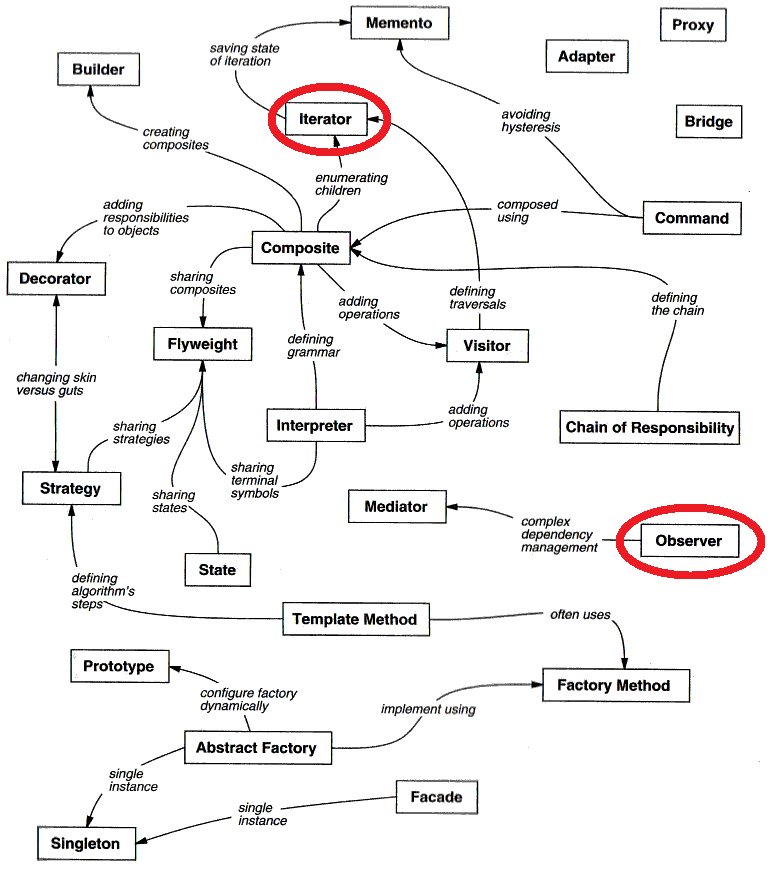
\includegraphics[width=0.48\textwidth]{figures/DesignPatternRelationships_bew.png}
	\end{center}
	\caption{Relations between design patterns according to \cite{gamma1994-DesignPatternsGOF}}
	\label{fig:designPatternRelationships}
\end{figure}

In 2010, a short paper called `\textit{Subject/Observer is Dual to Iterator}' \cite{meijer2010-Observable} was published by Erik Meijer, describing a mathematical relationship between the Observer pattern and the Iterator pattern based on categorical duality that had not been reported upon earlier. The paper shows that instances of the Observer pattern can be viewed as push-based collections, rather than the pull-based collections that result from the Iterator pattern. For later parts of this thesis, it is important to understand the mathematical basis of this relationship between the \obs and \obv interfaces in Rx and the \ieb and \ier interfaces in the Iterator pattern\footnote{For the purpose of the upcoming derivation we have chosen the C\# naming conventions of the Iterator pattern. In many other programming languages these interfaces are respectively known as \code{Iterable} and \code{Iterator}.} (see \Cref{lst:itb-itr}).

In most common languages \ieb forms the basis of the Collections API. It has only one method \code{getEnumerator} that returns the \ier to iterate over the elements in the collection. The \ier interface on the other hand contains two methods to be implemented: \code{moveNext} and \code{current}. The former performs a side effect by moving a pointer to the next element in the iteration and then returns a \code{Boolean} to indicate whether or not there was a next element. The latter is a pure function that just returns the element the pointer is currently pointing to. Notice that the \code{moveNext} method can throw an exception rather than returning \code{false} in case an error occurs.

Besides providing these two methods, \ier in \Cref{lst:itb-itr} also extends the \id interface. This interface is meant to signal to the \ieb that no more elements will be pulled and that it can `start collaborating' with the garbage collector to clean up resources. The real meaning of \ier extending \id however, is that \code{getEnumerator} not only returns an \ier, but also returns something that is disposable. The \id interface is therefore not really part of \ier but rather a part of what \code{getEnumerator} returns \cite{E2E-Rx}. For now we will consider \id to be a silent bystander that is will be ignored in the derivation.

\begin{minipage}{\linewidth}
\begin{lstlisting}[style=ScalaStyle, caption={\ieb and \ier interfaces}, label={lst:itb-itr}]
trait IEnumerable[T] {
    def getEnumerator(): IEnumerator[T]
}
trait IEnumerator[T] extends IDisposable {
    def moveNext(): Boolean // throws Exception
    def current: T
}
trait IDisplosable {
    def dispose(): Unit
}
\end{lstlisting}
\end{minipage}

These two interfaces together form the basis of all pull-based or interactive collections as described in \Cref{sec:reactive-programming}. The user asks for the next element and will get one in case a next element can be produced. In the following we will transform these interfaces for pull-based collections into interfaces for push-based or reactive collection, where the user subscribes to a collection and receives data once it is produced. This derivation, as well as its conclusion that interactive and reactive collections are each other's dual, is based on some categorical transformations and are discussed in several papers, as well as several keynotes and Channel9 video's \cite{meijer2010-Observable, meijer2012-YMIAD, E2E-Rx, meijer2014-Duality-And-The-End-Of-Reactive}. This derivation, as well as some of the intermediate steps are important for later parts of this thesis.

The first step in this derivation is to rewrite the two methods in the \ier interface into a single method \code{getNext()}. Using the categorical \textit{coproduct} \cite{rydeheard1988-Category-Theory} we can combine these two methods and determine its type signature: \code{getNext()} can either fail with an exception or succeed with either zero or one elements, resulting in the type signature \code{getNext(): Try[Option[T]]}. The new, intermediate, set of interfaces is shown in \Cref{lst:itb-itr-interm}.

\begin{minipage}{\linewidth}
\begin{lstlisting}[style=ScalaStyle, caption={\ier interface after applying coproduct}, label={lst:itb-itr-interm}]
trait IEnumerable[T] {
    def getEnumerator(): IEnumerator[T]
}
trait IEnumerator[T] {
    def getNext(): Try[Option[T]]
}
\end{lstlisting}
\end{minipage}

Since both interfaces now only have one single method, and given that the only purpose of \ieb is to produce an \ier, they can be written as a single lambda expression. An \ieb can be written as:

\begin{equation} \label{eq:itb}
\code{() $\Rightarrow$ (() $\Rightarrow$ Try[Option[T]])}
\end{equation}

Notice that applying \code{Unit} to the outer lambda yields another lambda expression, which corresponds to the type signature of \code{getNext} in \Cref{lst:itb-itr-interm}: \code{() $\Rightarrow$ Try[Option[T]]}.

The next step in this transformation is to dualize \cite{rydeheard1988-Category-Theory} lambda~expression~\ref{eq:itb}. A very informal way of describing duality is to flip all the arrows and rewrite the lambda expression. For example, the duality of $f :: A \rightarrow B$ is $\bar{f} :: A \leftarrow B \equiv B \rightarrow A$. In the same way, we can apply this to lambda~expression~\ref{eq:itb}, resulting in

\begin{equation} \label{eq:obs}
\code{(Try[Option[T]] $\Rightarrow$ ()) $\Rightarrow$ ()}
\end{equation}

This lambda expression takes a lambda \code{Try[Option[T]] $\Rightarrow$ Unit}, and returns \code{Unit}.

We can now put this lambda expression back into context by splitting it into two interfaces. The inner lambda \code{Try[Option[T]] $\Rightarrow$ ()} can be rewritten to an interface called \obv, which has one method \code{onNext(t: Try[Option[T]]): Unit}. This method can then be further rewritten into three separate methods by expanding the \code{Try[Option[T]]} type: \code{onNext(t: T): Unit}, \code{onError(e: Throwable): Unit} and \code{onCompleted(): Unit}. The outer lambda on the other hand translates to an interface called \obs, which has one method \code{subscribe(obv: Observer[T]): Unit}. Notice how these interfaces are completely identical to the ones presented in \Cref{lst:obs-obv}.

%So far the presence of \id has been ignored in this derivation. This interface can however be found in \Cref{lst:obs-obv}, renamed as \subs. \todo{Add a couple of words on the functionality of \id and \subs and how they are the same.}

So far, the presence of \id has been ignored in this whole derivation. The reason for that is that this interface is considered to be a \emph{second} thing that is returned by the \ieb, rather than a supertype of \ier. What therefore basically happened in the derivation is that we only dualized the enumerator\textit{ness} and left the disposable\textit{ness} out of the dualization process \cite{E2E-Rx}. Therefore the dualized \ier, now called \obv, still extends from \id, even though this only means that we pass \textit{two} arguments to the \code{Observable.subscribe(obv: Observer)}. Just as the \id was meant to signal to the \ieb that no more elements will be polled and that it can clean up its resources, now \id signals to the \obs that it should stop sending data to the \obv. Finally, \id is renamed to \subs and its method \code{dispose} is split into two methods \code{unsubscribe} and \code{isUnsubscribed}.

% really dualized the enumeratorNESS but not the disposableNESS
% \ieb returned \ier AND \id
% now we dualized the enumeratorNESS, \id remained, so we need to return \id in \obs instead of void
% so when we subscribe to an \obs with an \obv, we get back a \id to unsubscribe later

This derivation shows that interactive, pull-based collections are the mathematical dual of reactive, push-based collections. The \obs and \obv interfaces can directly be derived from the \ieb and \ier interfaces. Both sets of interfaces can therefore be considered to be collections. In other words: streaming data behaves exactly the same way as regular collections, such as arrays, lists and sets, except for them being push-based rather than pull-based \cite{meijer2012-YMIAD, meijer2010-Observable}. In the world of push-based collections one \emph{subscribes} to the stream in order to \emph{react} to the next element that is being send, whereas one \emph{asks} for the next element in a pull-based scenario.

\subsection{\obs as a monad}
\label{subsec:obs-monad}
As described in the previous section, \obs can also be written as lambda~expression~\ref{eq:obs}. A better look at this expression reveals that \obs is actually a special instance of the \textit{continuation monad}, which has the following type:

\begin{equation} \label{eq:cont}
\code{(S $\Rightarrow$ R) $\Rightarrow$ R}
\end{equation}

In the \obs lambda expression, \code{S} is equal to \code{Try[Option[T]]} and \code{R} is equal to \code{()} or \code{Unit}.

Given that \obs is just a continuation monad and hence an instance of \code{monad}, it automatically inherits the two operators that are defined on all monads: \code{return} and \code{(>>=)} (`bind'). In the Rx implementation, these operators are present as well. The \code{return} creates an \obs from a \code{Try[Option[T]]}, meaning that it accepts either an error, or an empty value, or a non-empty value. Therefore \code{return} is split into three operators \code{apply(t: T)}, \code{error(e: Throwable)} and \code{empty()}. Since an \obs can have multiple values, \code{apply} is overloaded to have more than one value. This overload was already shown in \Cref{subsec:core-comps}. The \code{(>>=)} operator is renamed to \code{flatMap} and also splits the \code{Try[Option[T]]} parameter into three separate parameters \cite{rx-api}. Besides that, since the \code{T $\Rightarrow$ Observable[S]} parameter is used most frequently, the \code{flatMap} operator is overloaded with only this parameter.

A simple example of using these monadic operators in Rx is shown in \Cref{lst:monad-in-rx}. On \cref{line:return} the overloaded \code{apply} is called, which lifts four values into the \obs. The \code{flatMap} operator on \cref{line:flatMap} doubles the number of elements by creating an \obs that emits the value as well as the square of the value.

\begin{minipage}{\linewidth}
\begin{lstlisting}[style=ScalaStyle, caption={Monad operators in Rx}, label={lst:monad-in-rx}]
Observable(1, 2, 3, 4) |\label{line:return}|
    .flatMap(x $\Rightarrow$ Observable(x, x * x)) |\label{line:flatMap}|
    .subscribe(x $\Rightarrow$ print(x + " "))

// result: 1 1 2 4 3 9 4 16
\end{lstlisting}
\end{minipage}

\subsection{Operators}
\label{subsec:operators}
In \Cref{subsec:derivation} we concluded that both the Iterator pattern and the Observer pattern are collections, only separated by the difference between push-based and pull-based behavior. All other rules on collections do however apply to both of them. In regular pull-based collections many operators are defined to manipulate, transform, filter, fold or group elements. These operators can therefore also be applied to push-based collections. One of them, \code{flatMap} was already shown in the previous section. However, rather than iterating over the pull-based collection and applying a transformation to each element, these operators \emph{react} to data being emitted by applying their particular transformation or side effect and passing the (transformed) data down to either a potential next operator or the \code{subscribe} method.

The Rx implementations of the \obs interface provide a wide variety of operators that apply all sorts of transformations to a data stream \cite{rx-api}. All operators are defined on \obs and will also return an \obs, making the API highly compositional. In order to understand how these operators work, we will look at some basic examples. Other, more advanced operators will be discussed in \Cref{subsec:avoiding-overproduction}.

\paragraph{Filter}To select only those elements that satisfy a certain predicate, the operator \code{filter(p: T $\Rightarrow$ Boolean): Observable[T]} is used. Every time an element is received by this operator, the predicate \code{p} will be applied. If the element satisfies the predicate, it is passed downstream; otherwise the element will be discarded. \Cref{lst:operators-obs} shows in \Cref{line:filter} how to select the odd numbers in a stream of integers by supplying a predicate.

\paragraph{Map}To transform one stream of data into another, the \code{map(f: T $\Rightarrow$ S): Observable[S]} is used. Each time an element (which is of type \code{T}) is received by this operator, the function \code{f} is applied to this element, yielding a new element of type \code{S}. This new element is then passed to down the stream. In \Cref{lst:operators-obs} the \code{map} operator is first applied in \cref{line:map} to the stream of filtered elements with a function that doubles the input.

\paragraph{Scan}Most operators do not allow for any form of internal state. They do not keep track of previous elements. An operator that can take the previous elements into account is \code{scan(seed: S)(acc: (S, T) => S): Observable[S]}. To this operator first of all a seed is supplied, which is the internal state of the operator before any value is received. Once an element is received, it will apply its internal state, together with that element to the accumulator function \code{acc} and produce an element to be emitted. This emitted value is also the new internal state of the operator. \Cref{lst:operators-obs} has a \code{scan} operator in \cref{line:scan} that takes the sum of all integers it receives and uses a \code{seed = 0}.

\paragraph{Drop}The \code{scan} operator is often used together with \code{drop(n: Int): Observable[T]}, which discards the first \code{n} elements and forwards all elements after that. The combination with the \code{scan} operator is used to prevent the seed value from being emitted further downstream, as is shown in \Cref{lst:operators-obs} \cref{line:drop}.

\paragraph{Take}Whereas \code{drop} discards the first \code{n} elements, \code{take(n: Int): Observable[T]} is used to only propagate the first \code{n} elements and discard all elements that come after that. In practice this means that the stream is terminated early with a call to \code{Observer.onCompleted()}. \Cref{lst:operators-obs} shows how \code{take} is used to only propagate the first and the second element and discard the third.

\begin{minipage}{\linewidth}
\begin{lstlisting}[style=ScalaStyle, caption={Operators on \obs}, label={lst:operators-obs}, columns=fixed]
Observable(1, 2, 3, 4, 5)		// emits:    1, 2, 3, 4,  5
    .filter(x $\Rightarrow$ x $\%$ 2 $==$ 1)			// emits:    1,    3,     5 |\label{line:filter}|
    .map(x $\Rightarrow$ x * 2)			// emits:    2,    6,    10 |\label{line:map}|
    .scan(0)((sum, x) $\Rightarrow$ sum + x)		// emits: 0, 2,    8,    18 |\label{line:scan}|
    .drop(1)				// emits:    2,    8,    18 |\label{line:drop}|
    .take(2)				// emits:    2,    8 |\label{line:take}|
    .subscribe(x $\Rightarrow$ println(x))
\end{lstlisting}
\end{minipage}

Just as the interactive collections, Rx has defined its operators in a way that composition of operators is very easy. In this way, simple operators can be chained in order to create the complex behavior that is often desired. There are many more operators defined on \obs, which are not mentioned in this section. For a full overview, we refer to the documentation on the Rx websites \cite{ReactiveX, rx-api, Rx.Net}.

\subsection{Different kinds of streams}
\label{subsec:stream-kinds}
There are many kinds of observable streams that can all be implemented using Rx. For example, a clock or a timer is basically a stream of `ticks' that emits an element every time unit and therefore has a constant speed. A stream of keyboard events on the other hand emits an element every time a key is pressed and therefore most likely has a very irregular speed. A data stream can also be the result of a database query or a network call. In these instances it might take a certain amount of time before the first result is emitted, but every other result is received almost immediately after the first result appeared.

%\subsubsection*{Finite vs. infinite}
Some of these data streams, like the database query, are finite and will at a certain time in the future call \code{onCompleted}. Others, like the clock, will keep producing next elements forever, be it at a regular pace or quite irregular, like the keyboard. This kind of stream will never call \code{onCompleted}, but still may terminate with an error by calling \code{onError}.

%There exist many operators in Rx to control these particular cases. Infinite streams can be limited by using operators like \code{take(n: Int)} (see \Cref{subsec:operators}), \code{takeUntil(predicate: T $\Rightarrow$ Boolean)} and \code{takeWhile(predicate: T $\Rightarrow$ Boolean)} that propagate all elements until or while a certain predicate is satisfied. Streams that terminate with an error can be resumed by operators like \code{retry()} or \code{onErrorResumeNext(resume: Throwable $\Rightarrow$ Observable[T])}, which respectively resubscribe to the same \obs or subscribe to another \obs.

%\subsubsection*{Hot vs. cold}
One other difference between certain streams is what happens when one subscribes multiple times to the same stream. Clocks or keyboard events, like broadcasters, emit values whether or not anyone is subscribed. If no one is subscribed, the events are still produced, but are immediately discarded. On the other hand, if multiple observers subscribe to the same stream, they will all receive the same events. This kind of stream is referred to as a \textit{hot} stream.

Some streams, like the \code{Observable(1, 2, 3, 4)} in \Cref{subsec:core-comps,subsec:obs-monad} or the database query, are not considered to be broadcasters. This kind of stream will create a new instance of itself every time an \obv subscribes to it. A second subscriber therefore receives the same result as a first subscriber, even though the second subscribes much later than the first one. This kind of stream is referred to as a \textit{cold} stream.

%A hot stream can be converted to a cold stream by sharing a single subscription with all observers. This can be done by operators like \code{share()} and \code{publish(f: Observable[T] $\Rightarrow$ Observable[S])}.

Notice that even though these differences do exist, they are not reflected in they type of the \obs. It is therefore always good to be careful with these distinctions and not to make any assumptions on streams being hot, cold, finite, infinite or error prone.

\subsection{Subjects}
\label{subsec:subjects}
A \subj can be viewed as a bridge between the \obv and the \obs. It can be subscribed to like an \obs, but can also observe another stream like an \obv. This is a very powerful tool that is often used as a starting point for a stream. Every time a certain event happens outside the context of the \subj, its \obv part can be called using the three methods. It will then process these events in its \obs part and propagate them down the stream.

A \subj can also be used to convert a cold stream into a hot stream. For this, a cold \obs is subscribed to the \subj. Because of this subscription, the cold \obs will be triggered to start emitting its events. The observable part of the \subj then becomes a hot \obs.

A special instance of \subj is the \bsubj, which behaves like a normal \subj but additionally emits its most recent value (or a seed or default value if none has been emitted yet) immediately after an \obv is subscribed to it. This is often used in user interface components like a text field to signal a certain initial state.

\subsection{Concurrency}
One final feature that makes Rx the `\textit{library for composing asynchronous and event based (reactive) programs}' is the way it handles concurrency. In most cases this is the hardest job for any developer and is often the cause of many bugs, deadlocks and race conditions. In Rx however, this is fully abstracted into two simple operators and one extra interface, resulting in a great API for switching from one thread to the other without introducing lots of extra code or bugs.

The first operator, called \code{observeOn(scheduler: Scheduler)}, propagates its received data in a Rx sequence to another thread. All mechanics of switching between threads is abstracted by the \sch, which takes workloads and schedules them on the thread it represents. By providing the \code{observeOn} a \sch, every bit of handling concurrency is done. This is shown in \Cref{lst:observeOn}, where an \obs emits the numbers 1 to 4 on the application's main thread, and where every number is doubled on that same thread. The \code{observeOn} operator, provided with a \code{NewThreadScheduler}, switches and propagates all data it receives to that \sch. All operations that are performed by both operators and \code{subscribe} methods after an \code{observeOn} is declared are switched to associated \sch.

One common use case of this operator is found in developing applications with a user interface (UI). When a textfield exposes an \obs of keyboard events, we may safely assume that it runs on the UI thread. The content of this textfield is transformed into a query, which is send of to a database, where it will collect and return a certain result set. While the database is processing the query, we do not want to block the UI thread, but rather keep that thread available for other, UI related processes. In this case it very useful to execute the database query on a different thread. For this purpose, RxJava provides a special IO \sch that is completely optimized for its cause. Once the result of the database query is received, a UI update needs to happen for the result to be shown. This can only be done from within the UI thread, hence the \obs needs to be switched back to that \sch using the \code{observeOn} operator.

\begin{minipage}{\linewidth}
\begin{lstlisting}[style=ScalaStyle, caption={\code{observeOn} in a Rx sequence}, label={lst:observeOn}]
Observable(1, 2, 3, 4)			// main thread
    .map(i $\Rightarrow$ 2 * i)			// main thread
    .observeOn(new NewThreadScheduler) |\label{line:observeOn-in-observeOn}|
    .map(i $\Rightarrow$ i / 2)			// thread 2
    .subscribe(i $\Rightarrow$ print(i + " "))	// thread 2
\end{lstlisting}
\end{minipage}

Something that is not possible with the \code{observeOn} operator is to schedule an \obs \textit{source} a different thread. For this purpose the \code{subscribeOn(scheduler: Scheduler)} is also part of the Rx API. This operator schedulers creation of all values within the source on the associated scheduler and also performs all operations on that \obs on the same \sch until a potential other \sch is encountered in the sequence of operator. This is described in \Cref{lst:subscribeOn}, where the creation of the values within \code{Observable.apply} is scheduled on a new thread. Compare this to \Cref{lst:observeOn}, where this was done on the application's main thread. Also the first \code{map} operation in \Cref{lst:subscribeOn} is performed on that same thread. When on \cref{line:observeOn-in-subscribeOn} the \code{observeOn} is encountered, the received data is rescheduled to a second thread.

\begin{minipage}{\linewidth}
\begin{lstlisting}[style=ScalaStyle, caption={\code{subscribeOn} in a Rx sequence}, label={lst:subscribeOn}]
Observable(1, 2, 3, 4)			// thread 1
    .subscribeOn(new NewThreadScheduler)
    .map(i $\Rightarrow$ 2 * i)			// thread 1
    .observeOn(new NewThreadScheduler) |\label{line:observeOn-in-subscribeOn}|
    .map(i $\Rightarrow$ i / 2)			// thread 2
    .subscribe(i $\Rightarrow$ print(i + " "))	// thread 2
\end{lstlisting}
\end{minipage}

More complex configurations of \code{subscribeOn} and \code{observeOn} can be made, as shown for example in \cite{RxJava-Scheduling}. Although very interesting, we consider these not relevant for the scope of this thesis. The main point here is that a stream can operate on different threads and that introducing concurrency is as easy as adding one line of code.